\documentclass{article}
\usepackage{graphicx}
\usepackage{float}
\usepackage{titlesec}
\usepackage{datetime}
\usepackage{geometry}
\usepackage{placeins}
\usepackage{minted}
\usepackage{xcolor}
\usepackage{listings}
\usepackage{caption}
\usepackage[document]{ragged2e}
\usepackage[hidelinks]{hyperref}
\usepackage{enumitem}
\geometry{
 a4paper,
 left=25mm,
 top=25mm,
 }
\captionsetup{hypcap=false} 
\newdateformat{daymonthyear}{\THEDAY .\THEMONTH .\THEYEAR}
\title{
  \centering
  
\includegraphics[width=\textwidth]{images/logo_PWr_kolor_poziom.png}\\
  \fontsize{28pt}{30pt}\selectfont Sprawozdanie 5\\
  \fontsize{14pt}{30pt}\selectfont Ćwiczenie 5.Teksturowanie}
\author{Krzysztof Zalewa}
\date{\daymonthyear\today}
\renewcommand*\contentsname{Spis treści}
\renewcommand{\figurename}{Rysunek}
\renewcommand{\listingscaption}{Fragment kodu}
\begin{document}
    \maketitle
    \pagebreak
    \tableofcontents
    \FloatBarrier
    \section{Wstęp teoretyczny}
        \subsection{Tekstury}
            Tekstura w OpenGL to obiekt który zawiera jeden lub więcej obrazów. Obiekt ten może zostać wykożystany
            w shaderach lub do renderowania obiektu. W OpenGL niezależnie od wielkości teksutry jej kordynaty 
            zawsze są w zakresie 0 - 1.
            \begin{figure}[ht]
                \centering
                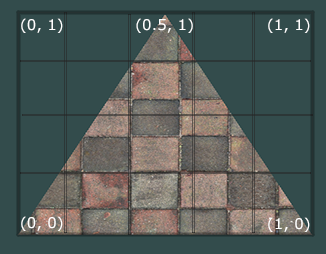
\includegraphics[width=0.5\textwidth]{images/tex_coords.png}
                \caption{Przykład kordynatów w OpenGL}
                \label{fig:coords}
            \end{figure}
            \pagebreak
        \subsection{Użyte tekstury}
        \raggedright
            Użyte tekstury pochodzą ze strony Dra. Gniewkowskiego(\hyperref[url:gniewkowski]{Źródła \ref{url:gniewkowski}})\linebreak
            \hyperref[fig:tex1]{\textbf{Tekstura \ref{fig:tex1}}} - To przykładowa tekstura\linebreak
            \hyperref[fig:tex2]{\textbf{Tekstura \ref{fig:tex2}}} - To plik \textbf{M1\_t.tga} z archwium tekstur\linebreak
            \hyperref[fig:tex3]{\textbf{Tekstura \ref{fig:tex3}}} - To plik \textbf{D8\_t.tga} z archwium tekstur\linebreak
            \begin{figure}[ht]
                \centering
                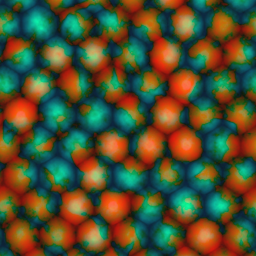
\includegraphics[width=0.5\textwidth]{images/tekstura1.png}
                \caption{Tekstura nr 1}
                \label{fig:tex1}
            \end{figure}
            \FloatBarrier
            \begin{figure}[ht]
                \centering
                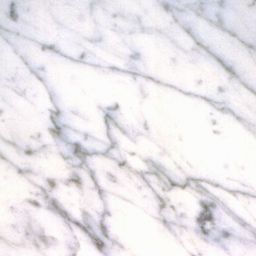
\includegraphics[width=0.5\textwidth]{images/tekstura2.png}
                \caption{Tekstura nr 2}
                \label{fig:tex2}
            \end{figure}
            \FloatBarrier
            \begin{figure}[ht]
                \centering
                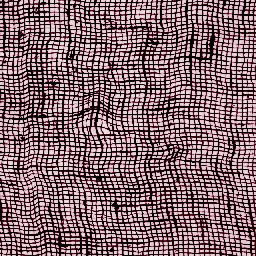
\includegraphics[width=0.5\textwidth]{images/tekstura3.png}
                \caption{Tekstura nr 2}
                \label{fig:tex3}
            \end{figure}
            \FloatBarrier
        \subsection{Funkcje w OpenGL}
            \raggedright
            \large{\textbf{\texttt{glGenTextures(1,\&textureIDs[texID])} - }} Generuje tablice 
            identyfikatorów tekstur\linebreak 
            \large{\textbf{\texttt{glBindTexture(GL\_TEXTURE\_2D,textureIDs[texID])} - }}Wybiera teksturę 
            o nr texID i przypisuje ją jako obecnie wybraną. Pozwala to na wykonywanie działań na
            tej teksturze (Przypisywanie konkretnej grafiki, rysowanie na obiekcie itd.)\linebreak 
            \large{\textbf{\texttt{glTexParameteri(GL\_TEXTURE\_2D,GL\_TEXTURE\_MIN\_FILTER,GL\_LINEAR)} - }}
            Definuje zachowanie tekstury gdy zostanie zrenderowana w skali mniejszej niż jej orginalny
            rozmiar. W tym przypadku \textbf{\texttt{GL\_LINEAR}} oznacza że tekstura jest interpolowana liniowo\linebreak 
            \large{\textbf{\texttt{glTexParameteri(GL\_TEXTURE\_2D,GL\_TEXTURE\_MAG\_FILTER,GL\_LINEAR)} - }}
            Definuje zachowanie tekstury gdy zostanie zrenderowana w skali większej niż jej orginalny
            rozmiar. Podobnie jak poprzednio \textbf{\texttt{GL\_LINEAR}} oznacza że tekstura jest interpolowana 
            liniowo\linebreak 
            \large{\textbf{\texttt{glTexParameteri(GL\_TEXTURE\_2D,GL\_TEXTURE\_WRAP\_S,GL\_REPEAT)} - }} 
            Ustawia tryb zapętlania tekstury w osi S (\textbf{\texttt{GL\_TEXTURE\_WRAP\_S}}) oś S to oś pozioma
            tekstury która odpowiada osi X obiektu. Opcja \textbf{\texttt{GL\_REPEAT}} oznacza że tekstura się 
            powtórzy. Np. Jeżeli trzeba wyświetlić teksturę w w punkcie \textbf{\texttt{S = 1.5}} to wyświetlona zostanie 
            tekstura w punkcie \textbf{\texttt{S = 0.5}} \linebreak 
            \large{\textbf{\texttt{glTexParameteri(GL\_TEXTURE\_2D,GL\_TEXTURE\_WRAP\_T,GL\_REPEAT)} - }} 
            Ustawia tryb zapętlania tekstury w osi S (\textbf{\texttt{GL\_TEXTURE\_WRAP\_T}}) oś T to oś pionowa
            tekstury która odpowiada osi X obiektu. Opcja \textbf{\texttt{GL\_REPEAT}} oznacza że tekstura się 
            powtórzy. Np. Jeżeli trzeba wyświetlić teksturę w w punkcie \textbf{\texttt{T = 1.5}} to wyświetlona zostanie 
            tekstura w punkcie \textbf{T = 0.5} \linebreak 
            \large{\textbf{\texttt{glTexImage2D(GL\_TEXTURE\_2D,0,GL\_RGB,width,height,0,GL\_RGB,GL\_UNSIGNED\_BYTE,data)} - }}
            Do wybranej tekstury przypisuje tablicę typu \textbf{\texttt{GL\_UNSIGNED\_BYTE}} (Wczytany obraz).
            Obraz ten ma rozmiary width*height i jego kolory zapisane są w formacie RGB\linebreak 
    \section{Zadanie laboratoryjne}
        \subsection{Treść zadania}
            W ramach zadania należało do poprzednio stworzonego programu dodać możliwość 
            teksturowania obiektów. Powinna być możliwość wyświetlenia trzech tekstur 
            głęboko strukturalnej, pośredniej i bez ustrukturyzowania. Program nie musi
            rysować obiektów za pomocą punktów i linii.
        \subsection{Opis działania programu}
            \raggedright
            Zgodnie z treścią zadania program rysuje 2 obiekty. Domyślnie 
            jajko i czajnik rysowane są w kolorze białym. Po wciśnięciu klawisza F3 lub F4
            zmieniana jest tekstura. Wyświetlone obiekty można obracać za pomocą myszki 
            (Przycisk musi być wciśnięty i zytrzymany). Program implementuje dwa światła 
            niebieskie i czerwone.\linebreak 
            \textbf{Kontrola obrotu:}\linebreak  
            \textbf{F1} - Tryb obrotu obiektu\linebreak
            \textbf{F2} - Tryb obrotu kamery\linebreak
            \textbf{F3} - Następna tekstura\linebreak
            \textbf{F4} - Poprzednia tekstura\linebreak
            \textbf{ESC} - Powrót do menu (okno konsolowe)\linebreak 
            \textbf{Ruch myszy w osi X} - Obrót kamery w osi X\linebreak 
            \textbf{Ruch myszy w osi Y} - Obrót kamery w osi Y\linebreak 
            \textbf{Scroll up} - Przybiliżenie obiektu\linebreak 
            \textbf{Scroll down} - Oddalenie obiektu\linebreak 
        \subsection{Kod programu}
            \begin{frame}
                \scriptsize
                \inputminted[
                    style={vs},
                    breaklines,
                    breakanywhere, 
                    linenos, 
                    tabsize=4 
                ]{c++}{Lab5.cpp}
                \vspace{1em}
                \captionof{listing}{Fragment kodu z programu}
                \label{lst:code}
            \end{frame}
            \begin{frame}
                \scriptsize
                \inputminted[
                    style={vs},
                    breaklines,
                    breakanywhere, 
                    linenos, 
                    tabsize=4 
                ]{c++}{Egg.cpp}
                \vspace{1em}
                \captionof{listing}{Kod Egg.cpp}
                \label{lst:egg}
            \end{frame}  
            \begin{frame}
                \scriptsize
                \inputminted[
                    style={vs},
                    breaklines,
                    breakanywhere, 
                    linenos, 
                    tabsize=4 
                ]{c++}{Light.cpp}
                \vspace{1em}
                \captionof{listing}{Kod Light.cpp}
                \label{lst:light}
            \end{frame}
    \section{Wnioski}
        Na zajęciach nie udało się dokończyć zadania. Po pracy w domu program działa poprawnie.
    \section{Źródła}
        \begin{enumerate}[label=\arabic*.]
            \item \url{https://learnopengl.com/Getting-started/Textures}
            \item \label{url:gniewkowski} \url{https://gniewkowski.wroclaw.pl/gk/}
            \item \url{https://www.khronos.org/opengl/wiki/texture}
        \end{enumerate}
\end{document}